\documentclass[dvipdfmx]{jsarticle}
\usepackage[papersize={10cm,5cm},margin=1mm,noheadfoot]{geometry}
\usepackage{tikz}
\usepackage[RPvoltages]{circuitikz}
\usepackage[nomessages]{fp}
\pagestyle{empty}

\begin{document}

\begin{figure}[htbp]
    \begin{center}
        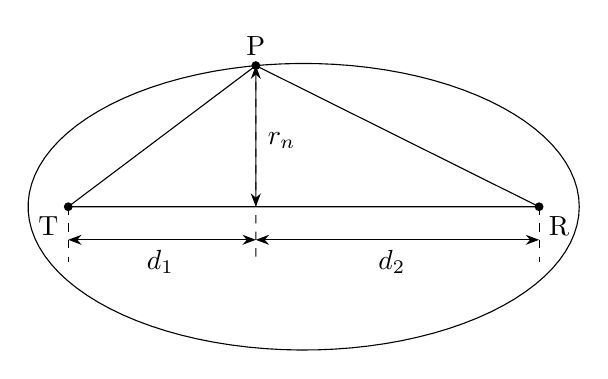
\begin{tikzpicture}[>=Stealth, scale=1.4]
            % 作図のための補助線
            % \draw[step=0.5, very thin, gray] (-2,-2) grid (2,2);
            % \draw[black, thick] (-2, 0) -- (2, 0);
            % \draw[black, thick] (0, -2) -- (0, 2);

            % 楕円の描画(x^2/a^2 + y^2/b^2 = 1)
            \FPeval{a}{2.5}
            \FPeval{b}{1.3}
            \FPeval{focal}{root(2, pow(2,\a)-pow(2,\b))}
            \draw[black, samples=100, variable=\th, domain=0:360] plot({\a*cos(\th)},{\b*sin(\th)});

            % 送信点、受信点の描画
            \coordinate (T) at (-\focal, 0);
            \coordinate (R) at (\focal, 0);
            \fill[black] (T) circle(0.04) node[anchor=north east] {T};
            \fill[black] (R) circle(0.04) node[anchor=north west] {R};

            % 点Pの描画
            \FPeval{pDeg}{100}
            \coordinate (P) at ({\a*cos(\pDeg)}, {\b*sin(\pDeg)});
            \fill[black] (P) circle(0.04) node[anchor=south] {P};

            % 距離
            \draw[black, <->] (-\focal, -0.3) -- ({\a*cos(\pDeg)}, -0.3);
            \draw[black, <->] (\focal, -0.3) -- ({\a*cos(\pDeg)}, -0.3);
            \draw[black, <->] (P) -- ({\a*cos(\pDeg)}, 0);

            % 補助線
            \draw[black, thin, dashed] (P) -- ({\a*cos(\pDeg)}, -0.5);
            \draw[black, thin, dashed] (T) --++ (0, -0.5);
            \draw[black, thin, dashed] (R) --++ (0, -0.5);
            \draw[black, thin] (T) -- (P) -- (R) -- cycle;
            \node at (-1.3, -0.5) {$d_1$};
            \node at (0.8, -0.5) {$d_2$};
            \node at (-0.2, 0.6) {$r_n$};
        \end{tikzpicture}
    \end{center}
\end{figure}

\end{document}
